\section{이탈 속도 (escape velocity)}

\pagestyle{headings}
\markboth{이탈 속도 (escape velocity)\hfill Kiehyun Park\hfill}



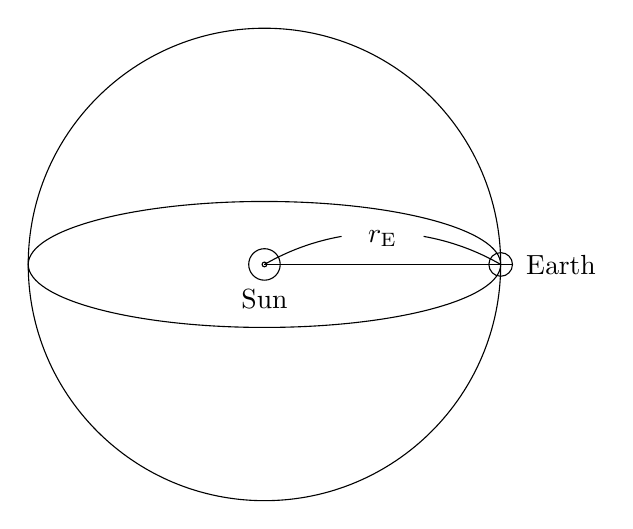
\begin{tikzpicture}[scale = 1, xshift = 1cm]
	\draw (5,2) circle (3cm);
	\draw (5,2) ellipse (3cm and 0.8cm);
	\draw (5,2) circle (0.03cm);
	\draw (5,2) circle (0.2cm) node[below, yshift=-0.2cm] {Sun};
	\draw (8,2) circle (0.15cm) node[right, xshift=0.2cm] {Earth};
	\draw (5,2) -- (8,2) node[above, xshift=-1.5cm, yshift=0.1cm] {$r_{\mathrm{E}}$};
	\draw (5,2) arc (120:100:3cm);
	\draw (8,2) arc (60:80:3cm);
	\draw (7.85,2) -- (8.15,2);
	\draw (8,1.85) -- (8,2.15);
\end{tikzpicture}

\vspace{1cm}
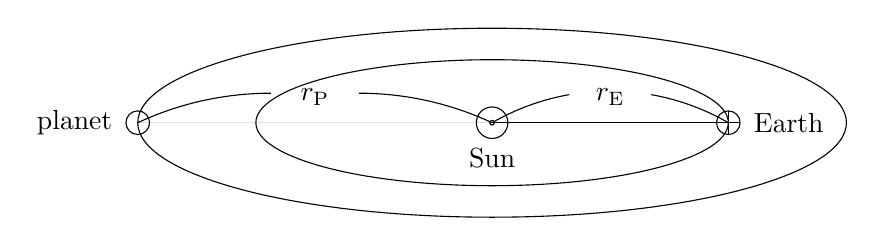
\begin{tikzpicture}[scale = 1, xshift = 1cm]
	\draw (5,2) ellipse (3cm and 0.8cm);
	\draw (5,2) ellipse (4.5cm and 1.2cm);
	\draw (5,2) circle (0.03cm);
	\draw (5,2) circle (0.2cm) node[below, yshift=-0.2cm] {Sun};
	\draw (8,2) circle (0.15cm) node[right, xshift=0.2cm] {Earth};
	\draw (5,2) -- (8,2) node[above, xshift=-1.5cm, yshift=0.1cm] {$r_{\mathrm{E}}$};
	\draw (5,2) arc (120:100:3cm);
	\draw (8,2) arc (60:80:3cm);
	\draw (0.5,2) circle (0.15cm) node[left, xshift=-0.2cm] {planet};
	\fill (5,2) -- (0.5,2) node[above, xshift=2.25cm, yshift=0.1cm] {$r_{\mathrm{P}}$};
	\draw (0.5,2) arc (115:90:4cm);
	\draw (5,2) arc (65:90:4cm);
	\draw (7.85,2) -- (8.15,2);
	\draw (8,1.85) -- (8,2.15);
\end{tikzpicture} 
	
\vspace{1cm}
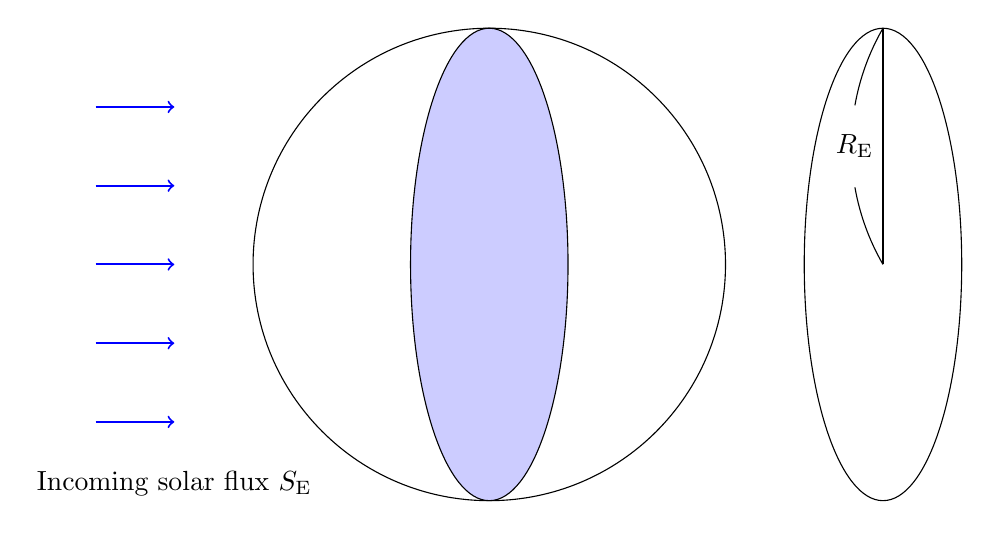
\begin{tikzpicture}[scale = 1, xshift = 1cm]
	\draw [line width=0.25mm, blue] [->] (0,0) -- (1,0) node[black, below, yshift=-0.5cm] {Incoming solar flux $S_{\mathrm{E}}$};
	\draw [line width=0.25mm, blue] [->] (0,1) -- (1,1);
	\draw [line width=0.25mm, blue] [->] (0,2) -- (1,2);
	\draw [line width=0.25mm, blue] [->] (0,3) -- (1,3);
	\draw [line width=0.25mm, blue] [->] (0,4) -- (1,4) ;
	
	\draw (5,2) circle (3cm);
	
	\fill [blue!20!white] (5,2) ellipse (1cm and 3cm) ;
	\draw (5,2) ellipse (1cm and 3cm) ;
	\draw (10,2) ellipse (1cm and 3cm);
	\draw (10,2) -- (10,5) node[left, yshift=-1.5cm] {$R_{\mathrm{E}}$};
	\draw (10,2) arc (210:190:3cm);
	\draw (10,5) arc (150:170:3cm);
\end{tikzpicture}

\begin{figure*}[h]
	\begin{tikzpicture}[rounded corners=3mm]
	\path node[rectangle,draw=green,fill=green!8,inner sep=.70cm] 
	{\parbox[t][15.5cm]{\textwidth-1.4cm-\fboxrule}
		{\question 
			행성 표면으로부터 고도 $h$에 있는 단위 질량인 물체의 이탈 속도를 구하시오.
			\begin{solutionorlines}[15cm]
			* 중력으로부터 물체가 탈출하는데 필요한 속도를 이탈 속도라고 하며 다음과 같이 구할 수 있다. 

			$ \dfrac{1}{2} m v_{\mathrm{e}}^{2} + \dfrac {- G M m}{r} = 0 $

			행성 대기의 상층부는 기체의 밀도가 낮으므로, 분자와 원자가 다른 분자나 원자와 충돌할 확률이 매우 적다 따라서 평균자유행로가 크며, 커다란 운동에너지를 가지므로 속도가 빨라 생성의 중력으로 부터 벗어나 외계로 이탈할 수 있다. 

			*   행성 표면으로부터 고도 $h$에 있는 단위 질량인 물체의 이탈 속도 : 

			$ v_{\mathrm{e}} = \sqrt {\dfrac{2Gm_{\mathrm{p}}}{r_{\mathrm{p}} + h}} $
			($G = 6.668\times10^{-11}\mathrm{kg^{-11} m^{3} s^{-2}}$)

			기체 분자에 이탈속도를 적용해 보자. 
			\end{solutionorlines}
	}};
	\end{tikzpicture}
\end{figure*}

\end{questions}
%(https://solarsystem.nasa.gov/system/resources/detail_files/681_ptemp.jpg)


# 맥스웰-볼츠만 분포

기체 분자들이 운동하고 있을 때 속도에 따른 분자 갯수는 맥스웰-볼츠만 분포를 따르게 되는데 이는 어떤 기체분자가 속도($v$)를 가질 확률이다. 

![대체 텍스트](http://www.kshitij-iitjee.com/Study/Physics/Part3/Chapter21/79.jpg)

위 그림을 보면 낮은 온도에서(파랑) 느린 분자가 압도적으로 많고, 빠른 기체분자는 거의 없다. 
높은 온도에서는(빨강) 빠른 분자가 많지만, 훨씬 완만한 분포를 가지며 느린 분자도 여전히 존재한다. 

분자들의 속력에 대한 멕스웰-볼츠만 분포는 아래와 같이 쓸 수 있다.

$f(v) = 4 \pi \left(\dfrac{M}{2\pi R T} \right)^{\frac{3}{2}} v^2 ~\mathrm{exp}\it \left[\dfrac{-Mv^2}{\rm{2} \it RT}\right]$

$f(v) = 4 \pi \left(\dfrac{m}{2\pi k T} \right)^{\frac{3}{2}} v^2 ~\mathrm{exp}\it \left[\dfrac{-mv^2}{\rm{2} \it kT}\right]$

($M$: 분자량, $m$: 분자의 질량)

최빈 속력($v_{\mathrm{mp}}$)는 $\dfrac{df(v)}{dv} = 0$으로 두고 $v_{mp}$에 대하여 풀면 

$v_{\mathrm{mp}} = \sqrt {\dfrac{2RT}{M}} = \sqrt {\dfrac{2kT}{m}}$

평균 속력은 속력 분포의 수학적 평균이므로 다음과 같이 된다.

${\overline{v}} = \int_{0}^{\infty} v f(v) dv = \sqrt {\dfrac{8kT}{\pi m}} = \sqrt {\dfrac{8RT}{\pi M}}$


또한 제곱 평균 속도, $v_{rms}$는 속력에 제곱하여 평균한 값에 제곱근을 취한 것이기 때문에 밑의 식으로 나타낼 수 있다.

$v_{\mathrm {rms} } = \sqrt {{\int _{0}^{\infty }v^{2}\, f(v)\, dv}} 
={\sqrt {\dfrac {3RT}{M}}}
= {\sqrt {\dfrac {3kT}{m}}}$

따라서 전체 속력은 아래와 같다.

$v_{\mathrm{mp}}<\overline{v} <v_{\mathrm {rms} }$


# 기체 분자 운동론

이상 기체를 가정하고 기체분자를 $x$, $y$, $z$ 방향중 $x$방향의 운동만 고려하면아래와 같이 모식할 수 있다.

![대체 텍스트](https://encrypted-tbn0.gstatic.com/images?q=tbn:ANd9GcRsHZTF-U5SpCHv93NAmYHiyoM8NwH9fKybymRd96oHcbaPhoFs)

$\Delta t$의 시간 동안 기체분자가 $2L$의 거리를 움직이므로 속도 $v$와 $\Delta t$는

$ v = \dfrac{2L}{\Delta t} $, $\Delta t = {2L}{v}$

완전탄성충돌을 가정했으므로 속도는 방향이 반대이고 크기가 같다. 따라서 운동량변화량은 

$\Delta P = mv - (-mv) = 2mv$

힘의 정의에서 다음과 같이 정리된다.

$F = \dfrac{\Delta P}{Delta t} = \dfrac{2mv}{\dfrac{2L}{v}} = \dfrac{2mv^2}{L}$

또한 압력의 정의에서

$ pressure = \dfrac{force}{area} = \dfrac{\dfrac{mv^2}{L}}{L^2} = \dfrac{mv^2}{L^3} = \dfrac {mv^2}{volume}$

1몰의 기체에 대해서는 아보가드로수를 곱해주고 보편기체상수$R$ 나누기 아보가드로수 $N_a$는 볼츠만 상수 $k$ 이므로 이상기체가정에 따라
$Pressure \times volyme = nRT - N_{A} mv^2$
$kT = mv^2$

운동에너지 정의에서

$E_{k, x} = \dfrac{1}{2} mv^2 = \dfrac{1}{2} kT$

분자는 $x$, $y$, $z$ 세 방향 모두 고려해주면
$E_{k} = E_{k, x} + E_{k, y} + E_{k, z} = \dfrac{3}{2} kT$

단원자기체가 아닌경우 분자의 회전운동을 고려해줘야 하기때문에

단원자 : $\dfrac{3}{2} kT$

이원자 : $\dfrac{5}{2} kT$

다원자 : $\dfrac{7}{2} kT$



# 이상 기체 상태 방정식

거시적인 이상 기체 상태 방정식은 다음과 같은 식으로 표현된다. 

*  $ PV = nRT $
($P$:압력, $V$:부피, $n$:기체의 몰수, $R$:기체 상수, $T$: 절대 온도)

실제 기체는 근사적으로 대개 이상 기체 법칙을 따르며, 기체의 밀도가 0에 가깝거나 기체의 온도가 매우 높으면 이상 기체 법칙에 더 잘 맞게 된다. 그 이유는 밀도가 0에 가까워지면 분자의 운동시 기체 분자끼리 부딪히는 정도가 적어지고 분자 자신의 부피를 무시할 정도가 된다. 또 고온이 됨으로써 분자의 운동이 고속이 되어 분자 간의 힘이 무시할 만한 정도가 되기 때문이다.

이를 미시적 관점에서 본 미시적인 이상 기체 법칙은 다음과 같다.

*  $ PV = N k T $
($P$:압력, $V$:부피, $N$:기체의 분자수, $k$:볼츠만 상수, $T$:절대 온도)

*  $ R = \dfrac{Nk}{n} $



# 행성의 대기


![대체 텍스트](http://ircamera.as.arizona.edu/astr_250/images/esc_vel.gif)

![대체 텍스트](https://i2.wp.com/mathscinotes.com/wp-content/uploads/2016/08/MolecularEscapeVelocity1.png)

기체분자론에 의하면 평균 분자 속도 ${\overline{v}}$ 가 갖는 운동에너지는 기체의 운동학적 온도 $T_{k}$ (kinetic temperature)와 분자의 질량($nm$)에 의해서 결정되므로 다음과 같이 나타낼 수 있다.

*  $ \dfrac{1}{2} m {\overline{v}}^{2} = \dfrac{3}{2} k T_{k}$

*  $ \overline{v} = \sqrt {\dfrac{3kT_{k}}{m}} $
($m$: 기체분자 1개의 질량, $k = 1.380658 \times 10^{23}\rm{J K^{-1}}$) 









